% We switch to portrait mode. This works as advertised.
\documentclass[a0,portrait]{a0poster}
% You might find the 'draft' option to a0 poster useful if you have
% lots of graphics, because they can take some time to process and
% display. (\documentclass[a0,draft]{a0poster})

\usepackage[margin=40mm]{geometry}

%\usepackage[utf8]{inputenc}

% Switch off page numbers on a poster, obviously, and section numbers too.
\pagestyle{empty}
\setcounter{secnumdepth}{0}

%fonts
\usepackage[T1]{fontenc}
\usepackage{kpfonts}
%\usepackage{roboto}
\usepackage{fontspec}
%\usepackage[oldstylenums, largesmallcaps]{kpfonts}
%\setmainfont[Numbers=OldStyle]{Tex Gyre Pagella}
\setmainfont{Tex Gyre Pagella}
\setsansfont[BoldFont=infini_bold,ItalicFont=infini_ital]{infini_romain}
%\setsansfont[BoldFont=Lovelo-LineBold]{Lovelo-LineBold}
%\setsansfont{Choplin-Medium-DEMO}
%\setsansfont{RobotoSlab-Bold}
%\setsansfont[StylisticSet=4]{MEgalopolisExtra}
%\renewcommand*\sfdefault{ugq}

\usepackage{hyperref}
\hypersetup{%
	pdftitle={Importance of many-body correlations in glass transition: an example from polydisperse hard spheres},%the title
	pdfauthor={Mathieu Leocmach},%your name
	hidelinks=true,
}

%proper math and math symbols
%\usepackage{amsmath}
\usepackage{amssymb}

\usepackage{siunitx}

\usepackage{tabu}
\usepackage{multirow}

% Allow the usage of graphics (.jpg, .png, etc.) in the document
\usepackage{graphicx}
\usepackage{tikz}
\usetikzlibrary{arrows,shapes,backgrounds, positioning, intersections, decorations.markings, decorations.shapes, mindmap, shapes.geometric, matrix, patterns}

\usepackage{pgfplots}
\pgfplotsset{compat=1.9}
\usepackage{pgfplotstable}
%\usepgfplotslibrary{units}
\usepgfplotslibrary{groupplots}
\pgfplotsset{every axis/.append style={xlabel near ticks,ylabel near ticks,mark size={0.2em}}}
\pgfplotsset{every axis plot post/.append style={very thick}}

\usepgfplotslibrary{external}
%\tikzexternalize
\tikzsetexternalprefix{fig_poster_palavas/}
\tikzset{external/system call={lualatex \tikzexternalcheckshellescape -halt-on-error -interaction=batchmode -jobname "\image" "\texsource"}}


\usepackage{ragged2e}
\RaggedRight

\usepackage{framed}
\colorlet{shadecolor}{lightgray!50!white}

\definecolor{Main}{rgb}{1, 0.57, 0}
\definecolor{Accent1}{rgb}{1,0.28,0}
\definecolor{Accent2}{rgb}{1,0.74,0}

% see documentation for a0poster class for the size options here
\let\Textsize\normalsize
\def\Norulehead#1{\noindent\hbox to \hsize{\hfil\LARGE\textcolor{Main}{\textsf{#1}}}\bigskip}
\def\Head#1{\Norulehead{#1\hrulefill}}
\def\LHead#1{{\LARGE #1}\smallskip}
\def\Subhead#1{\noindent{\large\color{Accent1}\textsc{#1}}}
\def\Title#1{\noindent{\VeryHuge\color{Accent2}\raggedright\textsf{
\addfontfeature{Ligatures=Rare}{#1}}}}

\renewcommand{\descriptionlabel}[1]{\hspace{\labelsep}\textcolor{Accent2}{\textsc{#1}}}

% The textpos package is necessary to position textblocks at arbitary 
% places on the page.
\usepackage[absolute,overlay,showboxes
]{textpos}
% Set up the grid
%
% Note that [40mm,40mm] is the margin round the edge of the page --
% it is _not_ the grid size. That is always defined as 
% PAGE_WIDTH/HGRID and PAGE_HEIGHT/VGRID. In this case we use
% 15 x 25. This gives us a wide central column for text (7 grid
% spacings) and two narrow columns (3 each) at each side for 
% pictures, separated by 1 grid spacing.
%
% Note however that texblocks can be positioned fractionally as well,
% so really any convenient grid size can be used.
%
\TPGrid[40mm,40mm]{15}{25}  % 3 - 1 - 7 - 1 - 3 Columns

% Mess with these as you like
\parindent=0pt
%\parindent=1cm
\parskip=0.5\baselineskip

\usepackage{paralist}

%bibliography
\usepackage{natbib}
\usepackage{bibentry}
\def\newblock{\hskip .11em plus .33em minus .07em}



\newlength{\mylength}

%\includeonly{}

\begin{document}
\pgfplotscreateplotcyclelist{earthy}{%
red!40!black,
red!60!black,
red!80!black,
red,
red!80!yellow,
red!60!yellow,
red!40!yellow,
}

\bibliographystyle{notitle}
%\nobibliography{sift}

% Understanding textblocks is the key to being able to do a poster in
% LaTeX. In
%
%    \begin{textblock}{wid}(x,y)
%    ...
%    \end{textblock}
%
% the first argument gives the block width in units of the grid
% cells specified above in \TPGrid; the second gives the (x,y)
% position on the grid, with the y axis pointing down.

% You will have to do a lot of previewing to get everything in the 
% right place.

% This gives good title positioning for a portrait poster.
% Watch out for hyphenation in titles - LaTeX will do it
% but it looks awful.


\begin{center}
\Title{
IMPORTANCE of MANY-BODY CORRELATIONS in GLASS TRANSITION: {\Huge an example from polydisperse hard spheres}
}
\end{center}

\vfill
\LHead{Mathieu Leocmach,\hfill \textsc{Laboratoire de Physique, Ecole Normale Supérieure de Lyon}
}\hfill\texttt{\color{Accent1}mathieu.leocmach@polytechnique.org}

\LHead{John Russo \& Hajime Tanaka\qquad
\textsc{Institute of Industrial Science, the University of Tokyo}
%\hfill\raisebox{0pt}[0pt]{
%	\includegraphics[height=2\baselineskip,clip=true, trim=6mm 14mm 6mm 0]{NEW-Logo-ERC-OUTLINE}\;
%	\includegraphics[height=2\baselineskip]{logo_ums_grand}\;
%	\includegraphics[height=2\baselineskip]{CNRSfilaire-Q}\;
%	\includegraphics[height=2\baselineskip]{CRPP}\;
%	\includegraphics[height=2\baselineskip]{logo_ens-lyon}
%}
}\\



\vfill
\begin{minipage}[t][21.5\TPVertModule]{11\TPHorizModule}
	\Head{Structure behind dynamic heterogeneities?}
	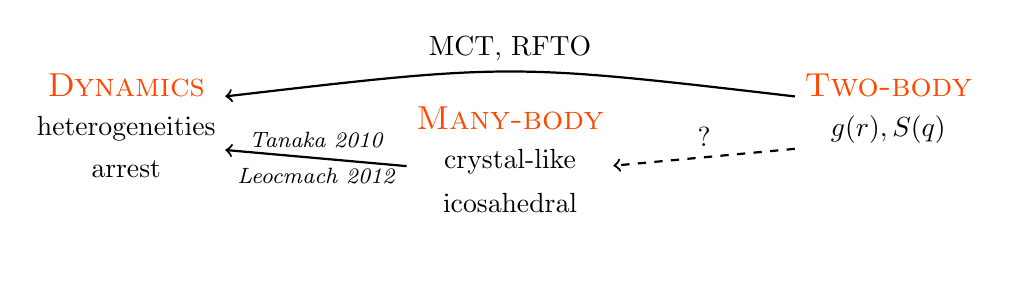
\begin{tikzpicture}
		\begin{scope}[every node/.style={rectangle split},every text node part/.style={font=\large\sffamily\scshape,Accent1}]
			\node (dyn) {Dynamics\nodepart{two}heterogeneities\nodepart{three}arrest};
			\node[anchor=base east] (twobody) at ($(dyn.base west) + (\textwidth,0)$) {Two-body\nodepart{two}$g(r), S(q)$};
			\node[anchor=north] (struct) at ($(dyn.base east)!0.5!(twobody.base west)$){Many-body\nodepart{two} crystal-like\nodepart{three}icosahedral};
		\end{scope}
		
		\draw[->, dashed, thick] (twobody) -- (struct) node[midway, above] {?};
		\draw[->, thick] (struct) -- (dyn)  node[midway, above, font=\footnotesize\itshape] {Tanaka 2010} node[midway, below, font=\footnotesize\itshape] {Leocmach 2012};
		\draw[->, thick] (twobody.base west) ..controls ($(struct.north)+(0,\baselineskip)$) .. (dyn.base east)  node[midway, above] {MCT, RFTO}; 
	\end{tikzpicture}
%	
%	Milk protein solution (4\%w sodium caseinate) acidified by the slow hydrolysis of glucono-$\delta$-lactone (\textsc{gdl})\\ \textit{Bremer et al., Colloids Surf. (1990); van Vliet \& Walstra, Faraday Discuss. (1995); Lucey \& Singh, Food Res. Int. (1997); Leocmach et al. PRL (2014)}
%	
%	\smallskip
%	\tikzsetnextfilename{prise_cas4}
%	\input{fig_poster_palavas/prise_cas4.pgf}
%	\begin{tabu}{X[5]XX[5]}
%	Caseins regain solubility below isoelectric $\Rightarrow$ overshoot in $G^\prime$&&
%	Single time scale $(t_m-t_i)$ governs gelation and softening.\\
%	How does it translate in term of microstructure?&&Diverge when $pH_\infty\rightarrow pI$
%	\end{tabu}
%	
%	\vfill
%	\Head{Linear rheology, from power-law to soft glassy}
%	\tikzsetnextfilename{sweep_cas4}
%	\input{fig_poster_palavas/sweep_cas4.pgf}
%	\begin{tabu}{X[4]X[2]X[5]}
%	Near isoeletric, power law rheology typical of gels.&&
%	Minimum in loss modulus appear with over-acidification.\\
%	Flatter with over-acidification.&%&
%	\multicolumn{2}{l}{\textcolor{Accent1}{$\blacktriangleright$} Over-acidified behaviour typical of soft glassy materials}\\
%	&\textit{Sollich, PRE (1998)}&\textit{Mason, Curr. Opin. Colloid Interface Sci. (1999)}\\
%	\end{tabu}
%	
%	\vfill
%	\Head{Evolution of the microscructure: preserved network, swelling aggregates}
%	\tikzsetnextfilename{structure_confocal}
%	\input{fig_poster_palavas/structure_confocal.pgf}
%	\begin{tabu}{X[5]XX[5]}
%	Maximum $G^\prime$ corresponds to maximum contrast between phases $\chi$&&
%	\textcolor{Accent1}{$\blacktriangleright$} Strongest gel when attraction is strongest\\
%	Characteristic size $\xi$ increases during over-acidification&&
%	\textcolor{Accent1}{$\blacktriangleright$} Casein aggregates swell $\sim$ over compressed gel $\Rightarrow$ soft glassy\\
%	\end{tabu}
%	
%	\vfill
%	\Head{Three creep regimes: much more erratic when over-acidified}
%	\tikzsetnextfilename{creep_cas4_gdl4}
%	\input{fig_poster_palavas/creep_cas4_gdl4.pgf}
%	\begin{tabu}{X[4]X[3]X[3]}
%	$\tau_f$: divergence of the strain $\gamma$, failure time&
%	\multicolumn{2}{l}{Robust Andrade creep, compatible with power-law rheology \hfill\textit{Leocmach et. al, PRL (2014)}}\\
%	$\tau_\text{min}$: minimum of shear rate $\dot{\gamma}$, fracture nucleation&
%	Robust finite time divergence&
%	\textcolor{Accent1}{$\blacktriangleright$}Possible to reform bonds? Glassy?
%	\end{tabu}
%	
%	
%	\vfill
%	\Head{Predict fracture nucleation time: Basquin law rescaling}
%	\begin{tabu}{XX}
%	\hspace{\TPHorizModule}\Subhead{Composition} rescaled by elastic modulus&
%	\hspace{\TPHorizModule}\Subhead{Geometry} rescaled as a fracture nucleation rate
%	\end{tabu}	
%	
%	\tikzsetnextfilename{basquin}
%	\input{fig_poster_palavas/basquin.pgf}
%	\begin{tabu}{X[5]XX[5]}
%	Robust Basquin law despite glassy behaviour&&\textcolor{Accent1}{$\blacktriangleright$} Failure determined by network breaking \& fracture nucleation
%	\end{tabu}
%	
\end{minipage}
%\hfill
%\begin{minipage}[b][21.5\TPVertModule]{3\TPHorizModule}
%\begin{shaded*}
%	\Norulehead{Take home}
%	\Subhead{Over acidification}
%	\begin{itemize}
%		\item protein aggregates swell
%		\item power-law rheology, decreasing exponent
%		\item dissipation becomes glassy
%	\end{itemize}
%	\Subhead{Creep response}
%	\begin{itemize}
%		\item Andrade creep
%		\item finite time singularity
%		\item erratic transition
%	\end{itemize}
%	\Subhead{Fracture time prediction}
%	\begin{itemize}
%		\item composition influence limited to $G^\prime$
%		\item geometry factors as a nucleation rate
%	\end{itemize}
%\end{shaded*}
%
%
%	\vfill
%	\Head{Microscopy}
%	Final state without over-acidification\\
%	
%	\tikzsetnextfilename{structure_finale}
%	\input{fig_poster_palavas/structure_finale.pgf}
%	
%	\vfill
%	\Head{Monkman-Grant}
%	Predict failure from the minimum
%	
%	\tikzsetnextfilename{MonkmanGrant}
%	\input{fig_poster_palavas/MonkmanGrant.pgf}
%	Height-dependent near isoelectric\\
%	Upper bound for over-acidified
%	
%	
%	\vfill
%	\Head{Wavelength}
%	\tikzsetnextfilename{lambda}
%	\input{fig_poster_palavas/lambda.pgf}
%	Compatible with nucleation rate
%	
%\end{minipage}
%
%\vfill
%\small{\texttt{The research leading to these results has received funding from the European Research Council under the European Union's Seventh Framework Programme (FP7/2007-2013) / ERC grant agreement n°~258803.}}
%
%





\end{document}